\chapter{情感分析系统}\thispagestyle{fancy}
为了更好地展示模型效果,本文实现了一套实时判断评论情感的展示系统。用户在前端输入语句后,该语句会通过网络传入系统服务器后台,进行分析,最后返回前端由网页展示。
\section{整体模块}
如图\ref{fmodule},系统主要分为两大模块即情感分析器和展示系统。情感分析器主要负责训练模型,预测输入文本的情感极性。展示系统包括服务器,前端网页和对应设计的RestAPI服务。整个系统由配置管理模块管理,以保证只需要改变参数就可以更改展示系统和模型参数,同时,配置管理模块也负责保存每次训练的模型参数,以便于记录和比较。
\begin{center}
\begin{figure}[!hbp]
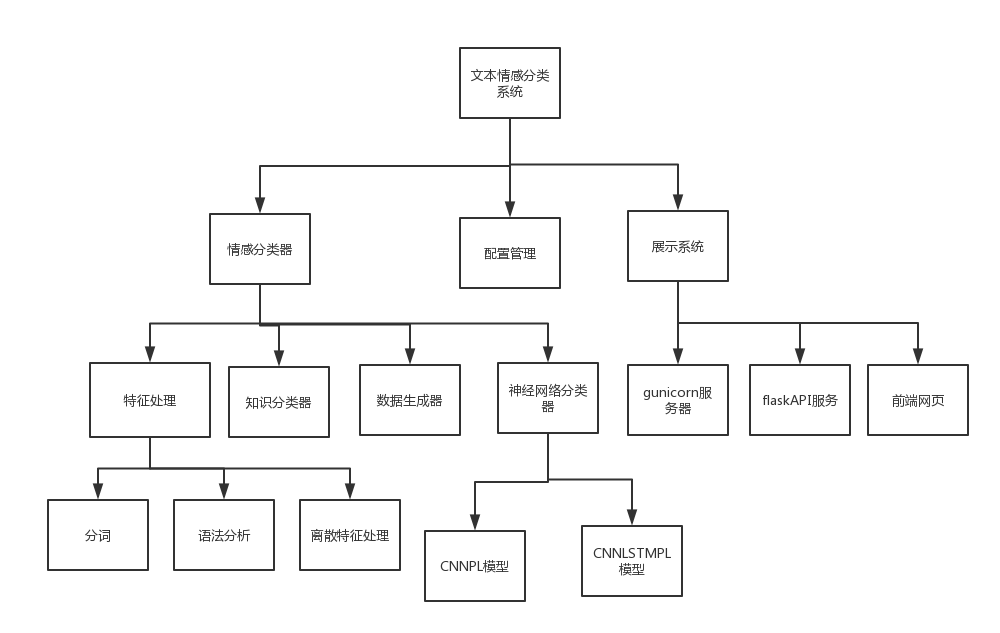
\includegraphics[width=\textwidth]{graphic/module.png}
\caption{系统基本模块图 \label{fmodule}}
\end{figure}
\end{center}
\section{开发环境}
\begin{enumerate}
\item 编程语言: Java, python
\item 开发环境: Eclipse, Pycharm
\item 依赖管理: pip, maven
\item 版本管理: git
\item 数据库: mongoDB
\item 架构: Restful API架构
\item Server: gunicorn
\item Restful API: flask
\item 前端:静态HTML + AJAX + JQuery + HTML5 + Bootstrap
\item 分词工具: Ansj, Stanford Parser
\item 英语词根化工具: nltk.stem.SnowballStemmer
\item 语法分析工具: Stanford Parser
\item 机器学习平台: tensorflow v1.1
\item java调用工具: jpype
\end{enumerate}